\section{Main Results}
\label{sec:results}

In this section, simulation analysis of the DMPC algorithm is provided. Implementation was done in MATLAB and executed on a PC with an Intel Xeon CPU and 16GB of RAM. The simulation parameters were $T = 15$s, $h = 0.2$s, $K = 15$ (3-second horizon), $r_{min} = 0.75$m and $a_{max} = -a_{min} = 0.7 [m/s^2]$. As for the penalty matrices, the values chosen were: $Q_{agg} = 1000I_3$, $Q_{coll} = 10I_3$, $S_{agg} = 10I_3$, $S_{coll} = 100I_3$, $R = I_3$. DMPC was allowed a maximum of 10 tries to converge.

\subsection{Four corner position exchange scenario}
To illustrate how DMPC is able to manage colliding trajectories, Fig.~(\ref{fig:four}) shows a transition problem for four vehicles, which were tasked to exchange positions in the plane. Initially, the agents follow a direct path towards their desired final locations, until future collisions are detected. In that moment, collision constraints start acting within the optimization problem, replanning the trajectories as to avoid the other vehicles. The constant replanning of trajectories allows the agents to coordinate and circumvent the congested area successfully. Such a cooperative behaviour is also observed in more difficult tasks (although harder to visualize), such as the one depicted in Fig.~(\ref{fig:30_random}), and is the key factor enabling large teams of vehicles to perform successful transitions.


\subsection{DMPC vs dec-iSCP}
To test the capabilities of the DMPC algorithm, we compared it to dec-iSCP \cite{chen2015decoupled}, a state-of-the-art algorithm using sequential convex programming. Scenarios with random sets of initial and final positions were generated and solved using both algorithms. The comparison criteria was the probability of success (finding feasible solutions within $T$ seconds) and the average computation time.

Fig.~(\ref{fig:comp_prob}) shows the probability of success as a function of the number of vehicles (ranging from 2 to 26). The proposed DMPC algorithm was able to find a solution in each case, whereas for dec-iSCP the amount of succeeded trials tended to decrease as the number of vehicles increased. The sequential solving nature of dec-iSCP makes it more difficult to solve as more vehicles are introduced to the problem, a shortcoming not experienced in DMPC thanks to the parallel nature of the algorithm.

\begin{figure}[t]
	\centering
	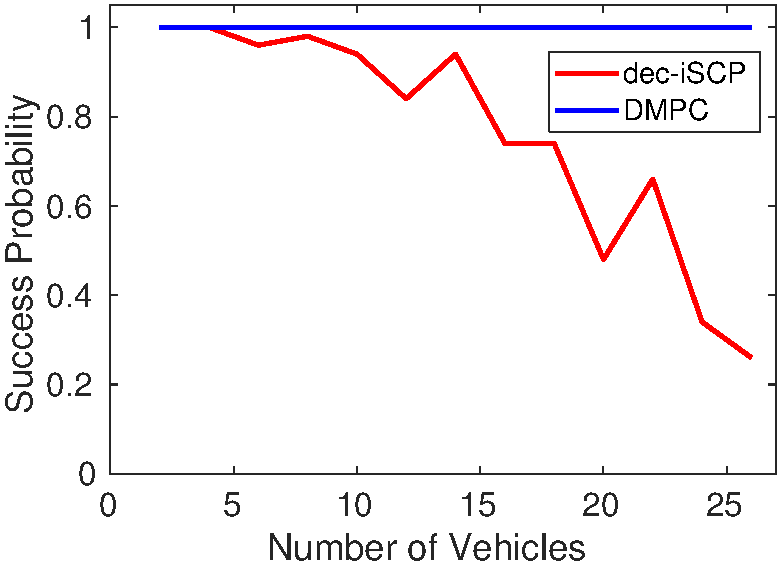
\includegraphics[width=0.4\textwidth]{figures/comp_prob}
	\caption{Probability of success comparison of DMPC and dec-iSCP, in a $5 \times 5 \times 2$ workspace. For every number of vehicles considered (2-26), 50 random initial and final positions were generated within the feasible set of the optimization problem, and solved using both algorithms. DMPC found a feasible solution in every case, while dec-iSCP failed for complex scenarios. }
	\label{fig:comp_prob}
\end{figure}

As for the computation time, Fig.~(\ref{fig:comp_time}) reveals that the complexity of the DMPC algorithm scales linearly with the number of vehicles. On the other hand, dec-iSCP seems to scale quadratically. Moreover, the standard deviation bars indicate there is a lot of variance in the computation time of dec-iSCP. The computational complexity of dec-iSCP is directly related with the number of collision constraints to be added for each vehicle \cite{chen2015decoupled}, which depends on the complexity of the transitions to execute. For DMPC, the variance in execution time is introduced mainly by the use of the heuristic approach, which sometimes forces the algorithm to recompute trajectories to find a solution. Naturally, as the number of vehicles increases, the difficulty of the transition also increases, which leads to a higher probability of DMPC requiring to recompute trajectories. This is seen in the increasingly larger standard deviation bars, although the variance is much less prominent than in dec-iSCP. Also, note that the MATLAB implementation of DMPC is unable to exploit the parallelization of the algorithm. A multi-threaded parallel implementation could significantly lower the runtimes shown in Fig.~(\ref{fig:comp_time}).


\begin{figure}[t]
	\centering
	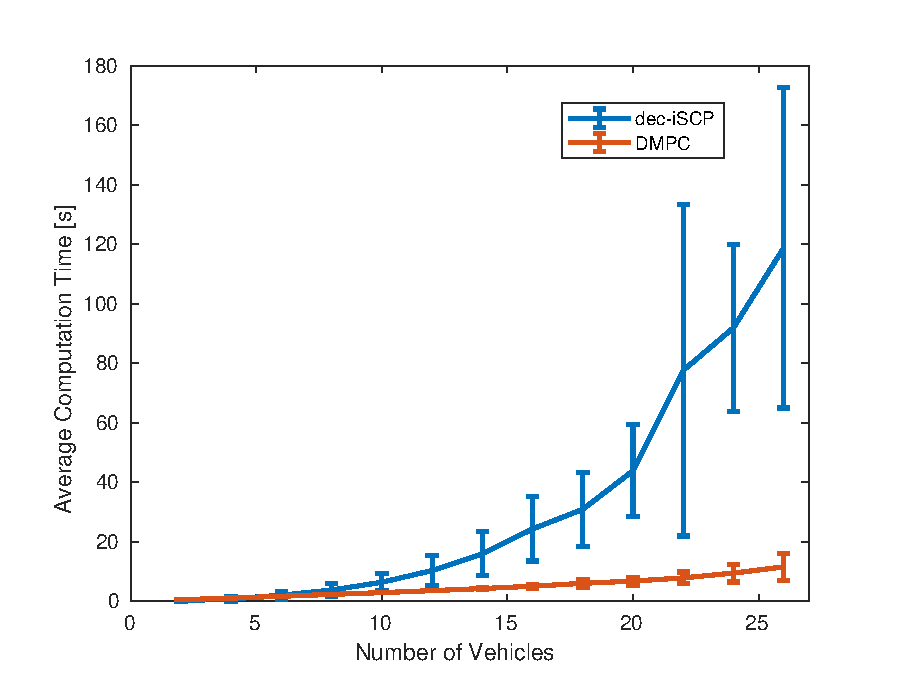
\includegraphics[width=0.4\textwidth]{figures/comp_time}
	\caption{Average computation time comparison of DMPC and dec-iSCP. Vertical bars denote one standard deviation form the mean. Results are for the same randomly generated trials as in Fig.~(\ref{fig:comp_prob}). DMPC drastically reduces average runtime and variance compared to dec-iSCP.}
	\label{fig:comp_time}
\end{figure}